\subsection{Algoritmo genético}
Para esta práctica se desarrolló un algoritmo genético que se apega al proceso mostrado en la Figura \ref{fig:AG}.

\begin{figure}[htbp]
	\centering
	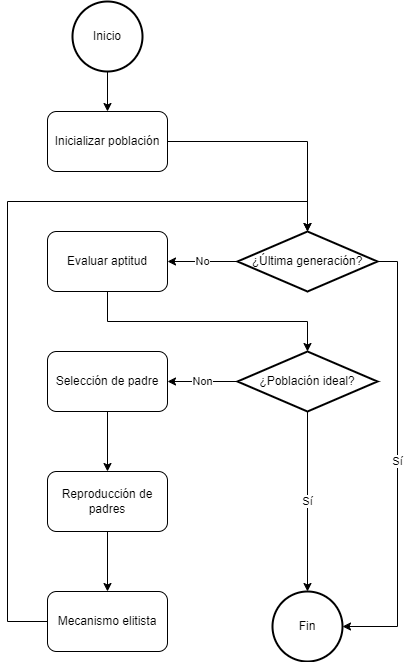
\includegraphics[width=0.5\textwidth]{algoritmo_genetico_proceso}
	\caption{Diagrama de flujo del algoritmo genético implementado.}
	\label{fig:AG}
\end{figure}

Para llevar a cabo dicho proceso, se optó por utilizar el lenguaje de programación Python, donde se diseñaron métodos genéricos para realizar los procesos de generación de población, evaluación de aptitud, selección de individuos, reproducción de individuos, mutación y mecanismos elitistas.


\subsection{Implementación en Python}
La implementación en Python se realizó siguiendo el procedimiento usual del algoritmo genético, agregando 2 modificaciones para manejar las restricciones:

\begin{itemize}
	\item Generación de población: Se utilizó el mecanismo de búsqueda tabú para garantizar que la población inicial contara con solamente individuos válidos.
	\item Previo a aplicar el mecanismo elitista, se diseñó un proceso en el cuál se penaliza con la suma de las distancias más grandes a cada uno de los individuos con combinaciones no válidas.
\end{itemize}


\subsection{Pruebas realizadas}
Se implementó una única combinación de mecanismos, el cuál incluye:

\begin{itemize}
	\item Selección monogamica.
	\item Cruza PMx.
	\item Mutación Scramble.
\end{itemize}

Dicha combinación de mecanismos se ejecutó en 5 ocasiones, esto para obtener un conjunto de soluciones posibles así como el promedio de la mejor distancia posible.

Cabe destacar que, dado que solamente se implementó 1 mecanismo elitista, este fue aplicado a todos los algoritmos por igual. También es importante mencionar que se implementó 1 criterio de paro:

\begin{itemize}
	\item Número de generaciones. Se estableció un límite de 10 generaciones para todos los algoritmos.
\end{itemize}
